\section{Design the control circuit using three variables: PWM, Direction, Brake as inputs}
\begin{figure}[H]
    \centering
    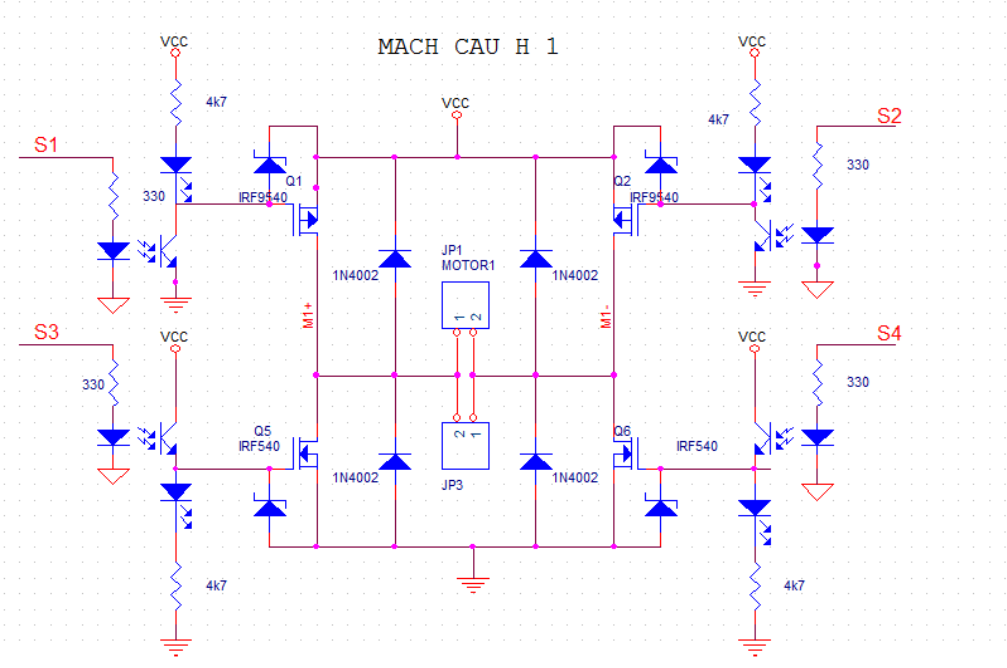
\includegraphics[width=\textwidth]{pictures/b3.png}
\end{figure}
\begin{tabular}{|c|c|c|c|c|c|c|c|}
    \hline
    PWM1 & PWM2 & BRAKE & S1 & S2 & S3 & S4 & TRANG THAI MOTOR \\
    \hline
    0 & 1 & 1 & 1 & 0 & 0 & 1 & QUAY CHIEU THUAN \\
    \hline
    0 & 0 & 1 & 0 & 1 & 1 & 0 & QUAY CHIEU NGHICH \\
    \hline
    X & X & 0 & 1 & 1 & 0 & 0 & THANG \\
    \hline
    1 & X & 1 & 0 & 0 & 0 & 0 & DUNG QUAY \\
    \hline
\end{tabular}
\subsection{Áp dụng bìa Karnaugh để tìm S1}
\begin{tabular}{|c|c|c|c|c|}
    \hline
    \diagbox{Z}{XY} & 00 & 01 & 11 & 10 \\
    \hline
    0 & 1 & 1 & 1 & 1 \\
    \hline
    1 & 1 & 1 & 0 & 0 \\
    \hline
\end{tabular}
$\Rightarrow S1 = \overline{Z} + \overline{X}.Y$ \\
\subsection{Áp dụng bìa Karnaugh để tìm S2}
\begin{tabular}{|c|c|c|c|c|}
    \hline
    \diagbox{Z}{XX} & 00 & 01 & 11 & 10 \\
    \hline
    1 & 1 & 1 & 1 & 1 \\
    \hline
    1 & 0 & 0 & 0 & 0 \\
    \hline
\end{tabular}
$\Rightarrow S2 = \overline{Z} + \overline{X}.\overline{Y}$ \\
\subsection{Áp dụng bìa Karnaugh để tìm S3}
\begin{tabular}{|c|c|c|c|c|}
    \hline
    \diagbox{Z}{XY} & 00 & 01 & 11 & 10 \\
    \hline
    0 & 0 & 0 & 0 & 0 \\
    \hline
    1 & 0 & 0 & 0 & 0 \\
    \hline
\end{tabular}
$\Rightarrow S3 = \overline{X}.\overline{Y}.Z$ \\
\subsection{Áp dụng bìa Karnaugh để tìm S4}
\begin{tabular}{|c|c|c|c|c|}
    \hline
    \diagbox{Z}{XY} & 00 & 01 & 11 & 10 \\
    \hline
    1 & 1 & 1 & 1 & 1 \\
    \hline
    0 & 0 & 0 & 0 & 0 \\
    \hline
\end{tabular}
$\Rightarrow S4 = \overline{X}.Y.Z$ \\